\clearpage
\section{Statistical interpretation}
\label{sec:Zprime_Limit}
Given that there are not evidence for a significant deviation from the SM expectations is observed, upper limits on the ratio of cross sections of a new resonance to the Z resonance are computed.

\subsection*{Methodology}
The statistical treatment of the results follows a Bayesian method with an unbinned extended likelihood function \cite{CMS-AN-16-307,StatsPaper,StatsWorkshop}. The mass range considered in the limit is a window of $\pm6\sigma$ with the window expanded symmetrically so it includes a minimum of 100 events. The barrel-barrel and barrel-endcap channels are treated as two separate channels and then combined together.
The probability density function (pdf) is modeled as the sum of a resonant signal pdf and a steeply falling background pdf as follows:
\begin{equation}
\label{eq:model_pdf}
f(m|\btheta,\bnu) = q_1 \cdot  f_\mathtt{S}(m|\btheta,\bnu)  + (1-q_1) \cdot  f_\mathtt{B}(m|\btheta,\bnu)
\end{equation}
where $m$ is the dilectron invariant mass, \btheta\ is the vector of parameters of interest and \bnu\ the vector of nuisance parameters. The probability of a signal event is given by $q_1$.
The signal pdf $f_{S}$ is modeled as a Breit-Wigner convoluted with a resolution function $\mathrm{Res}(m | \sigma ,\btheta)$:
\begin{equation} \label{eq:sigpdf}
f_{\mathrm{S}} (m | \Gamma, \sigma, \btheta, \bnu) = \mathrm{BW}(m | \Gamma) \otimes \mathrm{Res} (m | \sigma ,\btheta, \bnu)
\end{equation}
where $\Gamma$ is the intrinsic width of the signal and $\sigma$ is the mass resolution.
As described in Section \ref{sec:mass_res} the resolution function $\mathrm{Res}(m | \sigma ,\btheta, \bnu)$ is described by a Cruijff (double-sided crystal ball) function in 2016 (2017).

The background pdf $f_{B}$ has instead an ad-hoc shape derivation computed using simulated background events. An analytic function is used to describe the background shape in the search region above 140 GeV of dielectron invariant mass and it can be expressed by:
%\begin{equation}\label{eq:bkgshape}
%f_{B}(m| a, b, c, d, k) = e^{a+b\times m+c\times m^2+d\times m^3}m^{k}
%\end{equation}\begin{linenomath*}

\begin{equation}
\begin{split}
m^{\kappa}\mathrm{exp}(\sum\limits_{i=0}^3 \alpha_{i} m^{i}), \mbox{if }m \le \mbox{600 GeV} \\
m^{\lambda}\mathrm{exp}(\sum\limits_{i=0}^3 \beta_{i} m^{i}), \mbox{if }m > \mbox{600 GeV,}
\end{split}
\label{eq:bkgshape}
\end{equation}

The parameters is determined by a fit to the simulated dielectron mass spectrum.
The background spectra together with the fitted function are shown in Figure \ref{fig:bkgFits} for the barrel-barrel and barrel-endcap categories.


\begin{figure}
  \begin{center}
    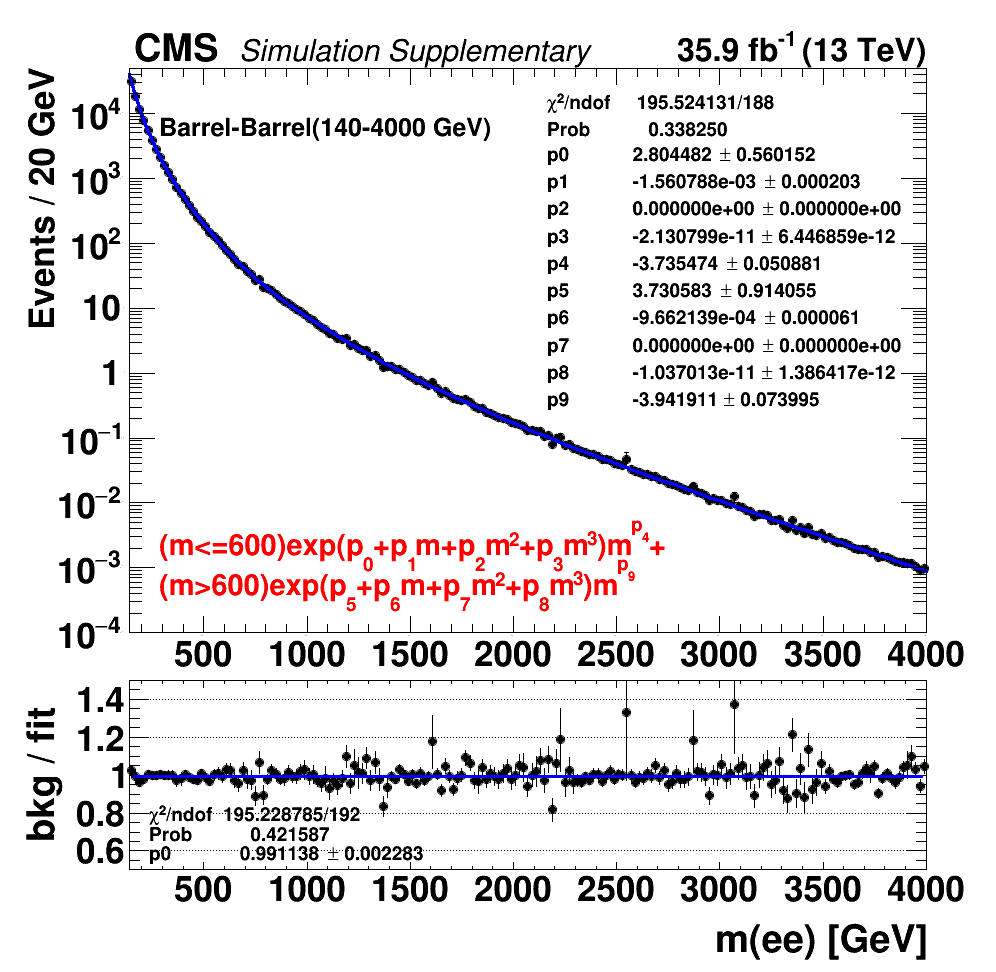
\includegraphics[width=0.47\textwidth]{figures/Zprime/2016/bgkfit/BB_140_4000_bgk.png}
    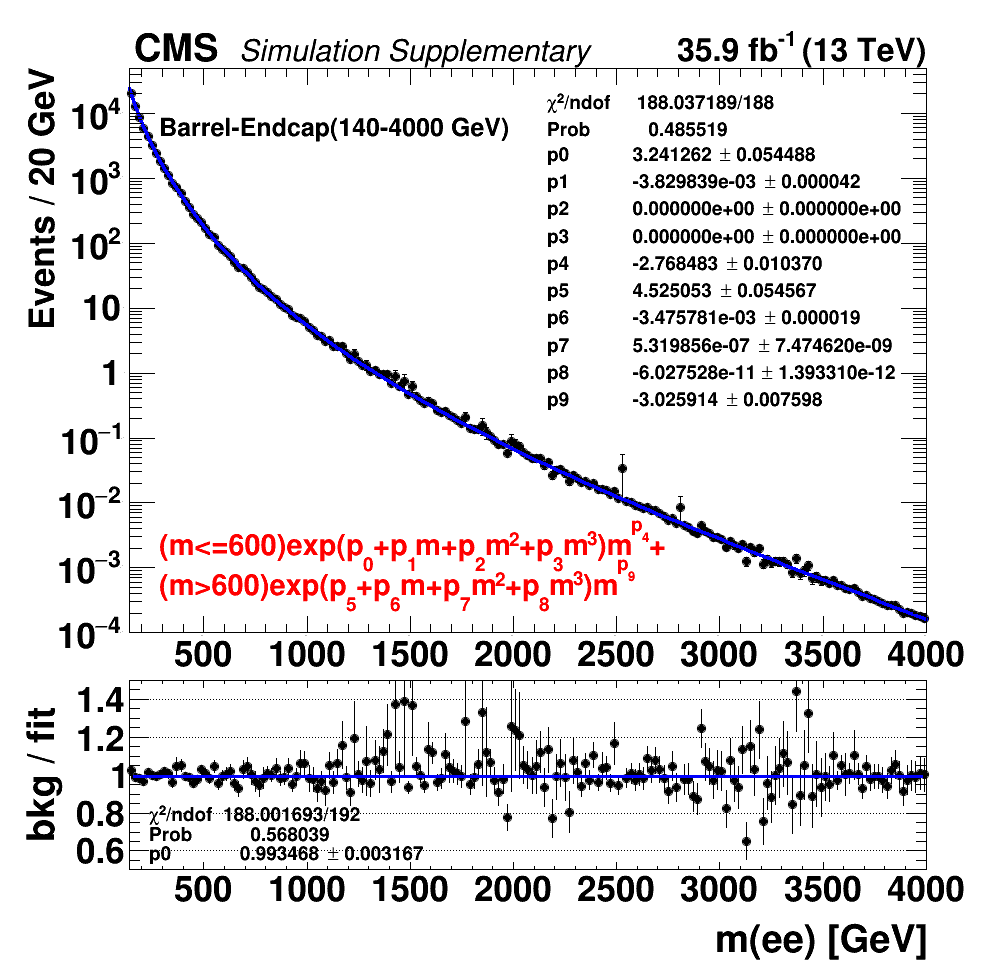
\includegraphics[width=0.47\textwidth]{figures/Zprime/2016/bgkfit/BE_140_4000_bgk.png}
    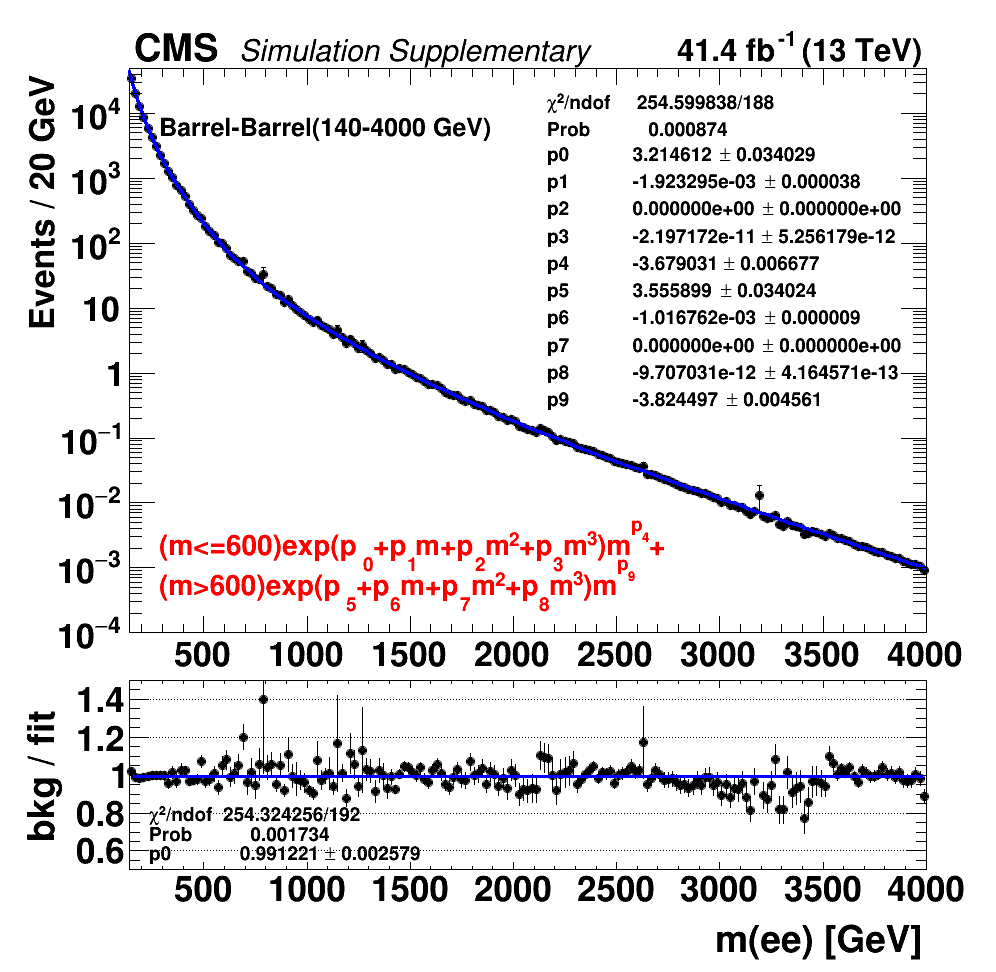
\includegraphics[width=0.47\textwidth]{figures/Zprime/2017/bgkfit/BB__bgk.png}
    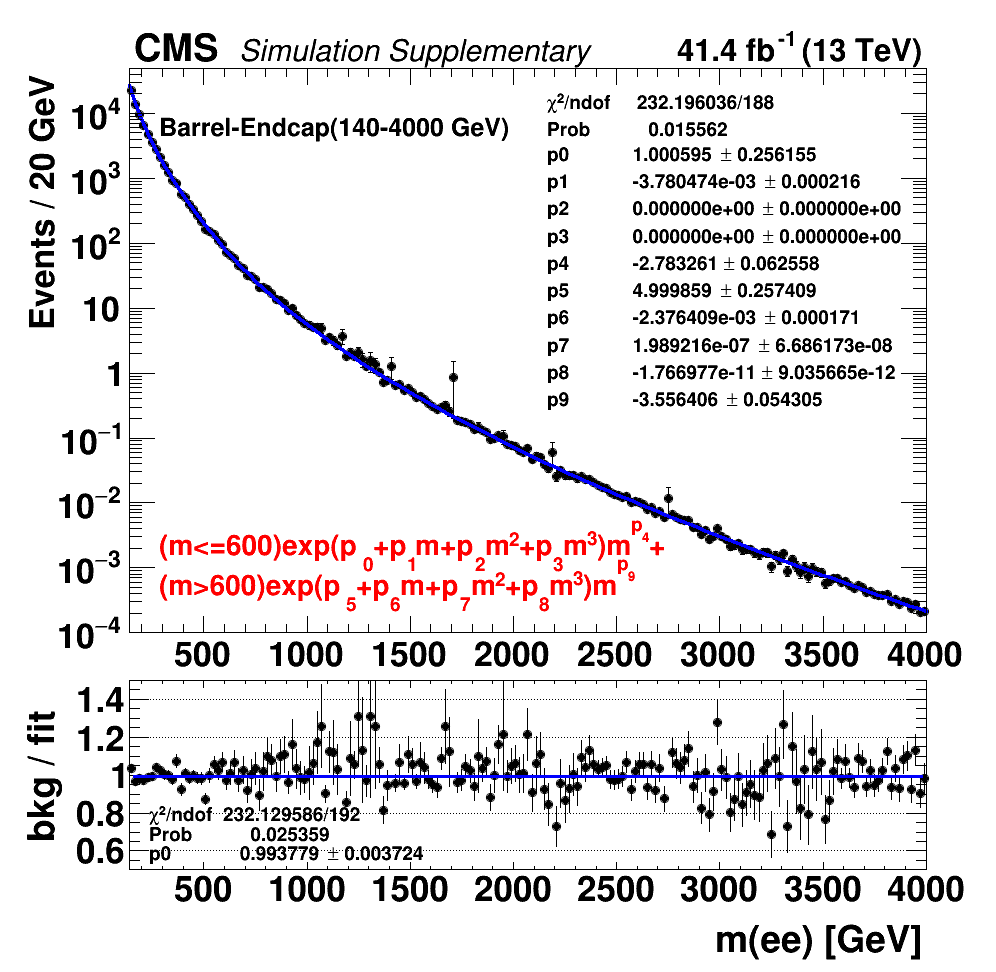
\includegraphics[width=0.47\textwidth]{figures/Zprime/2017/bgkfit/BE__bgk.png}
    \caption{The total SM background together with the fitted functional form used to enter it into the limit setting tools for the barrel-barrel (left) and barrel-endcap (right) channels in 2016 (top) and 2017 (bottom).}
    \label{fig:bkgFits}
  \end{center}
\end{figure}

The unbinned likelihood is defined as:
\begin{eqnarray}
\label{like}
 \mathcal{L}\left( \bm \vert R_\sigma, \bnu \right) & = & \prod_{i=1}^{N} f\left(m_i \vert R_\sigma, \bnu \right)
\end{eqnarray}
where the product is over the events in the dataset and \bm\ is the vector of corresponding dielectron masses and the $R_\sigma$ is the parameter of interest in this analysis, defined as the ratio between the cross section times branching ratio (BR) to electron pairs of a generic new resonance and the same quantity for the Z resonance in the mass region 60-120 GeV:
\begin{equation}
R_{\sigma}=\frac{\sigma_{\mathrm{Z^{'}}}\cdot\mathrm{BR(Z^{'}\rightarrow ee)}}{\sigma_{\mathrm{Z}}\cdot\mathrm{BR(Z\rightarrow ee)}}
\end{equation}
This choice has the important advantage that certain uncertainties, e.g. the uncertainty on the integrated luminosity or any other \ET-independent effect will be canceled out or are at least greatly reduced.
Proceeding in extending the likelihood with a poissonian normalization component in front of equation (\ref{like}) and inserting the equation for the signal and background pdfs detailed above, one obtains:
\begin{equation}
\mathcal{L}(\bm|R_\sigma,\bnu) =
  \frac{\mu^Ne^{-\mu}}{N!} \cdot
    \prod_{i=1}^{N}
      \left(
        \frac{\mu_\mathrm{S}(R_\sigma,\bnu)}{\mu}f_\mathrm{S}(m_i|R_\sigma,\bnu)
        + \frac{\mu_\mathrm{B}(R_\sigma,\bnu)}{\mu}f_\mathrm{B}(m_i|R_\sigma,\bnu)
      \right)
      \label{eq:ext_likelihood}
\end{equation}
with $\mu_{\mathrm{S}}$ and $\mu_{\mathrm{B}}$ being the signal and background yields and $\mu$ the sum of the two yields.
The $R_{\sigma}$ can be connected to the signal event yield $\mu_{\mathrm{S}}$ via the following relation:
\begin{equation}
\label{eq:musig}
\mu_{\mathrm{S}} = R_\sigma \frac{(\mathrm{Acc}\times\epsilon)_{\mathrm{Z}^{'}}}{(\mathrm{Acc}\times\epsilon)_{\Z}} N_{\Z}
\end{equation}
where $(\mathrm{Acc}\times\epsilon)_{\mathrm{Z}^{'}}$ and $(\mathrm{Acc}\times\epsilon)_{\Z}$ are the acceptance times efficiency of the $\mathrm{Z^{'}}$ (shown in Figure \ref{fig:accEff}) and the Z boson respectively and $N_{\Z}$ is the number of selected Z events, defined in the mass region 60-120 GeV.



The uncertainties on the nuisance parameters in the vector \bnu\ are taken into account by modeling the nuisance parameter as
\begin{equation}
\label{eq:nu}
\nu = \hat{\nu} \cdot (1 + \delta\nu)^{\beta}
\end{equation}
where $\hat{\nu}$ is the estimate of $\nu$, $\delta\nu$ is the corresponding systematic uncertainty and $\beta$ is a random number drawn from a gaussian distribution with mean value at zero and second order moment equal to 1 (denoted as $Gauss(\beta|0,1)$). The likelihood is then weighted by $Gauss(\beta|0,1)$ for each nuisance parameter giving
\begin{equation}
\mathcal{L}( \bm \vert R_\sigma, \bnu) = \mathcal{L}( \bm \vert R_\sigma, \bnu\ )\cdot \prod_{j}Gauss(\beta_j|0,1)
\end{equation}
where the product is done over the nuisance parameters. The two categories of the analysis are independent categories, hence the total likelihood can be obtained by multiplying the two separated likelihoods. With this definition of the likelihood function, 95\% confidence level (CL) upper limits can be computed using the Bayes theorem, which states:
\begin{equation}
f(R_\sigma,\bnu|\bm) \cdot p(\bm) =
\mathcal{L}(\bm|R_\sigma,\bnu) \cdot p(R_\sigma,\bnu)
\end{equation}
where $p(R_\sigma,\bnu)$ is the prior pdf for the parameter of interest of the model. In this analysis, the prior is taken as a log-normal distribution for the uncertainties, and a uniform (positive) prior for the parameter of interest. After integrating over the nuisance parameters $\bnu$, one obtains
\begin{equation}
p(R_\sigma|\bm) \cdot p(\bm) =
\mathcal{L}(\bm|R_\sigma) \cdot p(R_\sigma)
\end{equation}
The expression for the posterior pdf immediately follows as
\begin{equation}
p(R_\sigma|\bm) =
  \frac{\mathcal{L}(\bm|R_\sigma) \cdot p(R_\sigma)}{p(\bm)} =
  \frac{\mathcal{L}(\bm|R_\sigma) \cdot p(R_\sigma)}{\int\mathcal{L}(\bm|R_\sigma) \cdot p(R_\sigma)\,\mathrm{d}R_\sigma}
\end{equation}
Given the posterior pdf for the parameter of interest $R_\sigma$,
the 95\% C.L. upper limit $R_\sigma^{95}$ is defined by the following constraint:
\begin{equation}
\label{eq:ul}
\int_0^{R_\sigma^{95}}p(R_\sigma|\bm)\,\mathrm{d}R_\sigma = 0.95
\end{equation}
where the integration is done using the Metropolis-Hasting algorithm~\cite{Metropolis,HASTINGS01041970}.

Finally, it is worth to mention that (see Equation (\ref{eq:musig})) the parametrization of the acceptance times efficiency $(\mathrm{Acc}\times\epsilon)_{\mathrm{Z}^{'}}$ is shown in figure~\ref{fig:accEff}. Other inputs required for the limit setting tool are listed in table~\ref{tab:limitInput}, as well as the number of data events and acceptance at the Z peak region. Since the limits are normalised to the Z peak, any $E_T$ independent effects on the efficiency cancel and are not included in the acceptance times efficiency parametrisation nor the Z peak acceptance x efficiency. The effects not included are the data/MC efficiency scale factor and the trigger ID efficiency.
The uncertainty for $(\mathrm{Acc}\times\epsilon)_{\mathrm{Z}^{'}}/(\mathrm{Acc}\times\epsilon)_{\mathrm{Z}}$ is mainly due to data/MC HEEP selection scale factor at high $\ET$ as well as NLO and PDF effects on the Drell-Yan background. A 2\% (1\%) energy scale uncertainty is assigned for barrel-barrel (barrel-endcap) channel.

\begin{figure}
  \begin{center}
    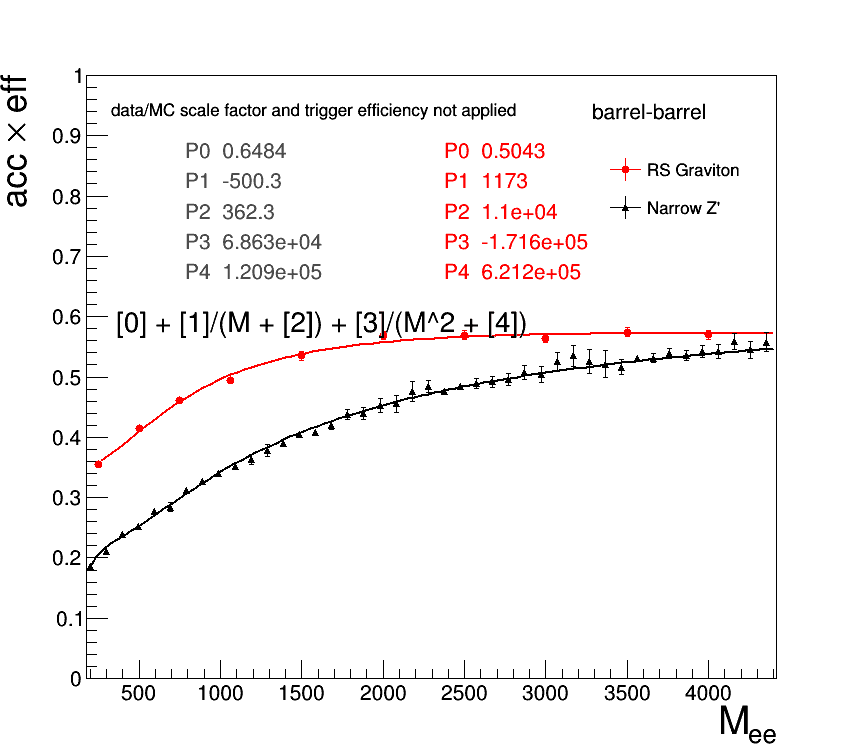
\includegraphics[width=0.47\textwidth]{figures/Zprime/2016/limitInputs/plot_acceff_BB.png}
    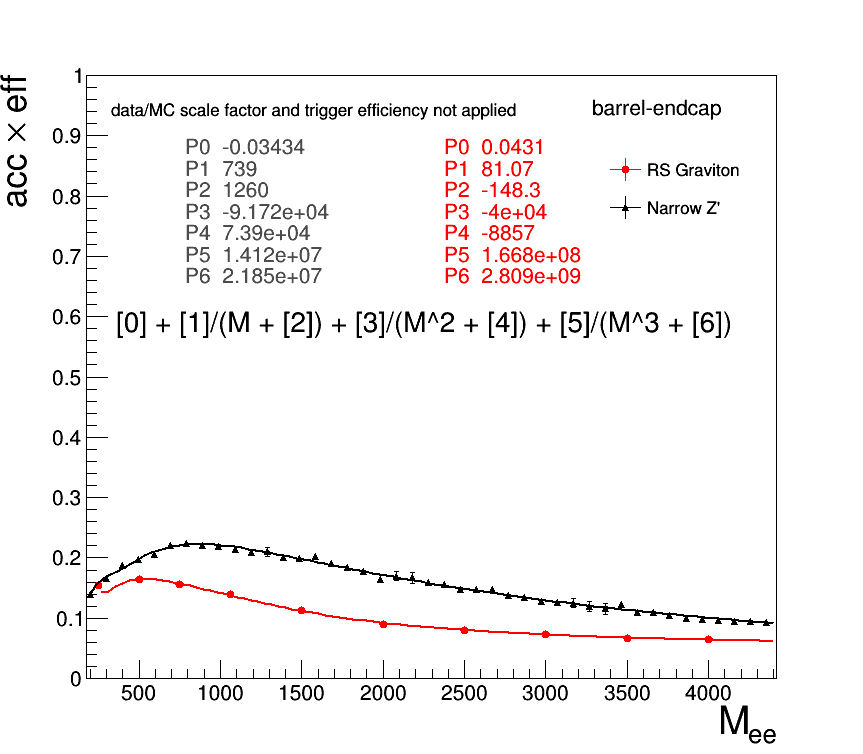
\includegraphics[width=0.47\textwidth]{figures/Zprime/2016/limitInputs/plot_acceff_BE.png}
    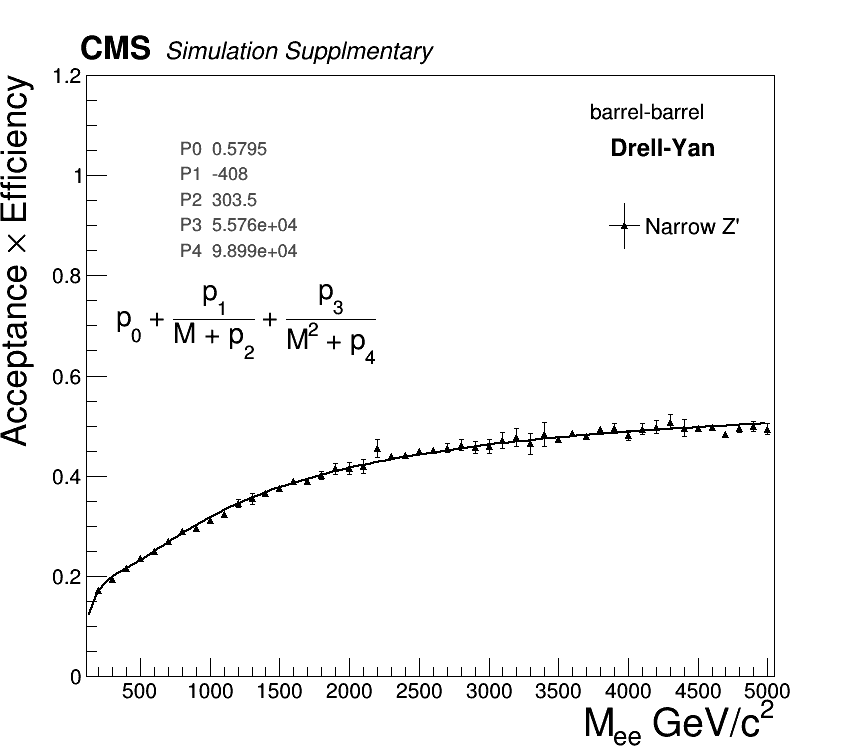
\includegraphics[width=0.47\textwidth]{figures/Zprime/2017/limitInputs/plot_acceff_BB.png}
    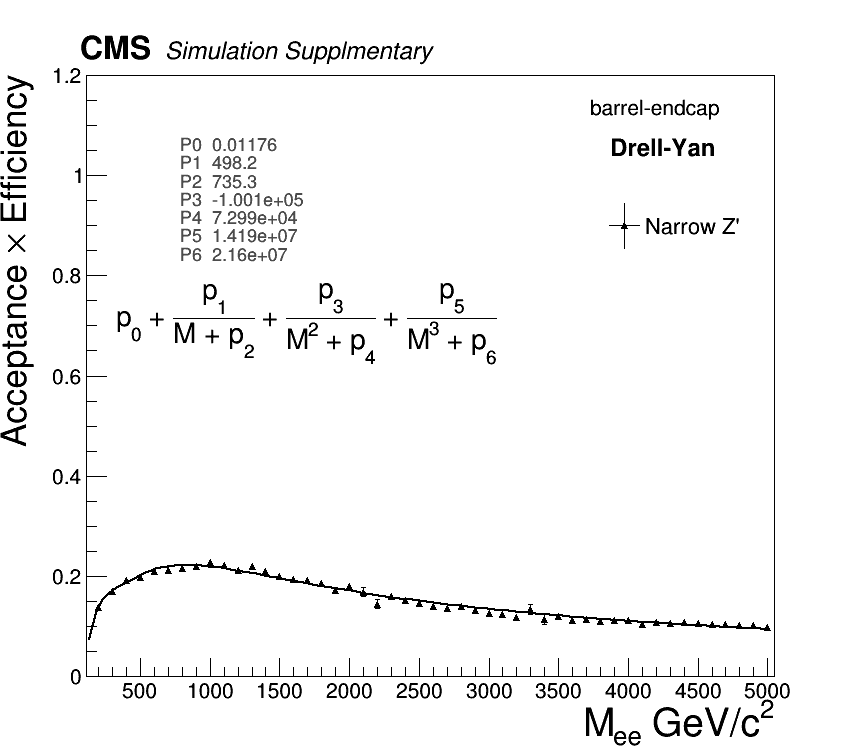
\includegraphics[width=0.47\textwidth]{figures/Zprime/2017/limitInputs/plot_acceff_BE.png}
    \caption{The acceptance times efficiency of for a spin-1 or spin-2 particle to be selected by the analysis in the barrel-barrel region (left) and barrel-endcap region(right) together with the fitted functional form used to enter it into the limit setting tools in 2016 (top) and 2017 (bottom). $E_T$ independent effects which will cancel in the ratio to the acceptance times efficiency at the Z peak are not included. These are primarily the data/MC efficiency scale factor and the trigger ID efficiency.}
    \label{fig:accEff}
  \end{center}
\end{figure}

\begin{table} [t]
\begin{center}
\begin{tabular}{|c|c|c|c|} \hline
Year                 &Variable                                 & EB-EB   & EB-EE \\\hline
\multirow{4}{*}{2016}&$N_{Z}$ (60-120 GeV)                     & 5730976 & 2042478 \\
                     &$(\mathrm{Acc}\times\epsilon)_{\mathrm{Z}}$ (60-120 GeV)            & 0.0895  & 0.0318 \\
                     &$(\mathrm{Acc}\times\epsilon)_{\mathrm{Z}^{'}}/(\mathrm{Acc}\times\epsilon)_{\mathrm{Z}}$ err & 6\%     & 8\%\\
                     &energy scale uncertainty                 &  2\%    & 1\% \\ \hline
\multirow{4}{*}{2017}&$N_{Z}$ (60-120 GeV)                     & 6156571 & 2086010 \\
                     &$(\mathrm{Acc}\times\epsilon)_{\mathrm{Z}}$ (60-120 GeV)            & 0.0811  & 0.0294 \\
                     &$(\mathrm{Acc}\times\epsilon)_{\mathrm{Z}^{'}}/(\mathrm{Acc}\times\epsilon)_{\mathrm{Z}}$ err & 6\%     & 8\%\\
                     &energy scale uncertainty                 &  2\%    & 1\% \\ \hline
\end{tabular}
\caption{The input parameters to the limit setting code. The MC efficiencies do not have the data/MC scale factor applied or any $E_{T}$ independent efficiency like HLT identification efficiency although $E_T$ dependent effects like L1 and HLT turn on are included.}
\label{tab:limitInput}
\end{center}
\end{table}

\subsection*{Expected limits}
Expected upper limits on $R_\sigma$ under the background-only hypothesis are obtained by computing the median of a set of limits derived using an ensemble
of randomly drawn pseudo-data. The limits for the pseudo-data are
estimated using the same procedure as described for the observed limits. The pseudo-data are generated by drawing the event yield as a random number from a Poisson distribution whose mean is
\begin{equation}
\label{eq:exp_mu}
\mu_{B} = \hat{\mu}_{B} \cdot (1 + \delta\mu_{B})^{\beta_{B}}
\end{equation}
where $\beta_{B}$ is again a random number extracted from a normal distribution as the case of Equation (\ref{eq:nu}). The value of $\hat{\mu}_{B}$ is estimated by integrating
the background shape over the observable range, where the shape is normalized over a sideband in the data below 200 GeV of dielectron invariant mass.
Repeating this procedure many times, the distribution of the expected limits under the background-only hypothesis is built, therefore the median and the $\pm1\sigma$ and $\pm2\sigma$ bands of the limit can be computed.


\subsection{Upper limits}
Using the method described above, the observed and expected 95\% upper limits on $R_\sigma$ for a resonance width of 0.6\% is shown in Figure ~\ref{fig:limit_ee}.
The signal $R_{\sigma}$ curves are shown on the plot in order to obtain a mass limit on two specific $\mathrm{Z}^{'}$ signal model.

\begin{figure}[!htb]
\centering
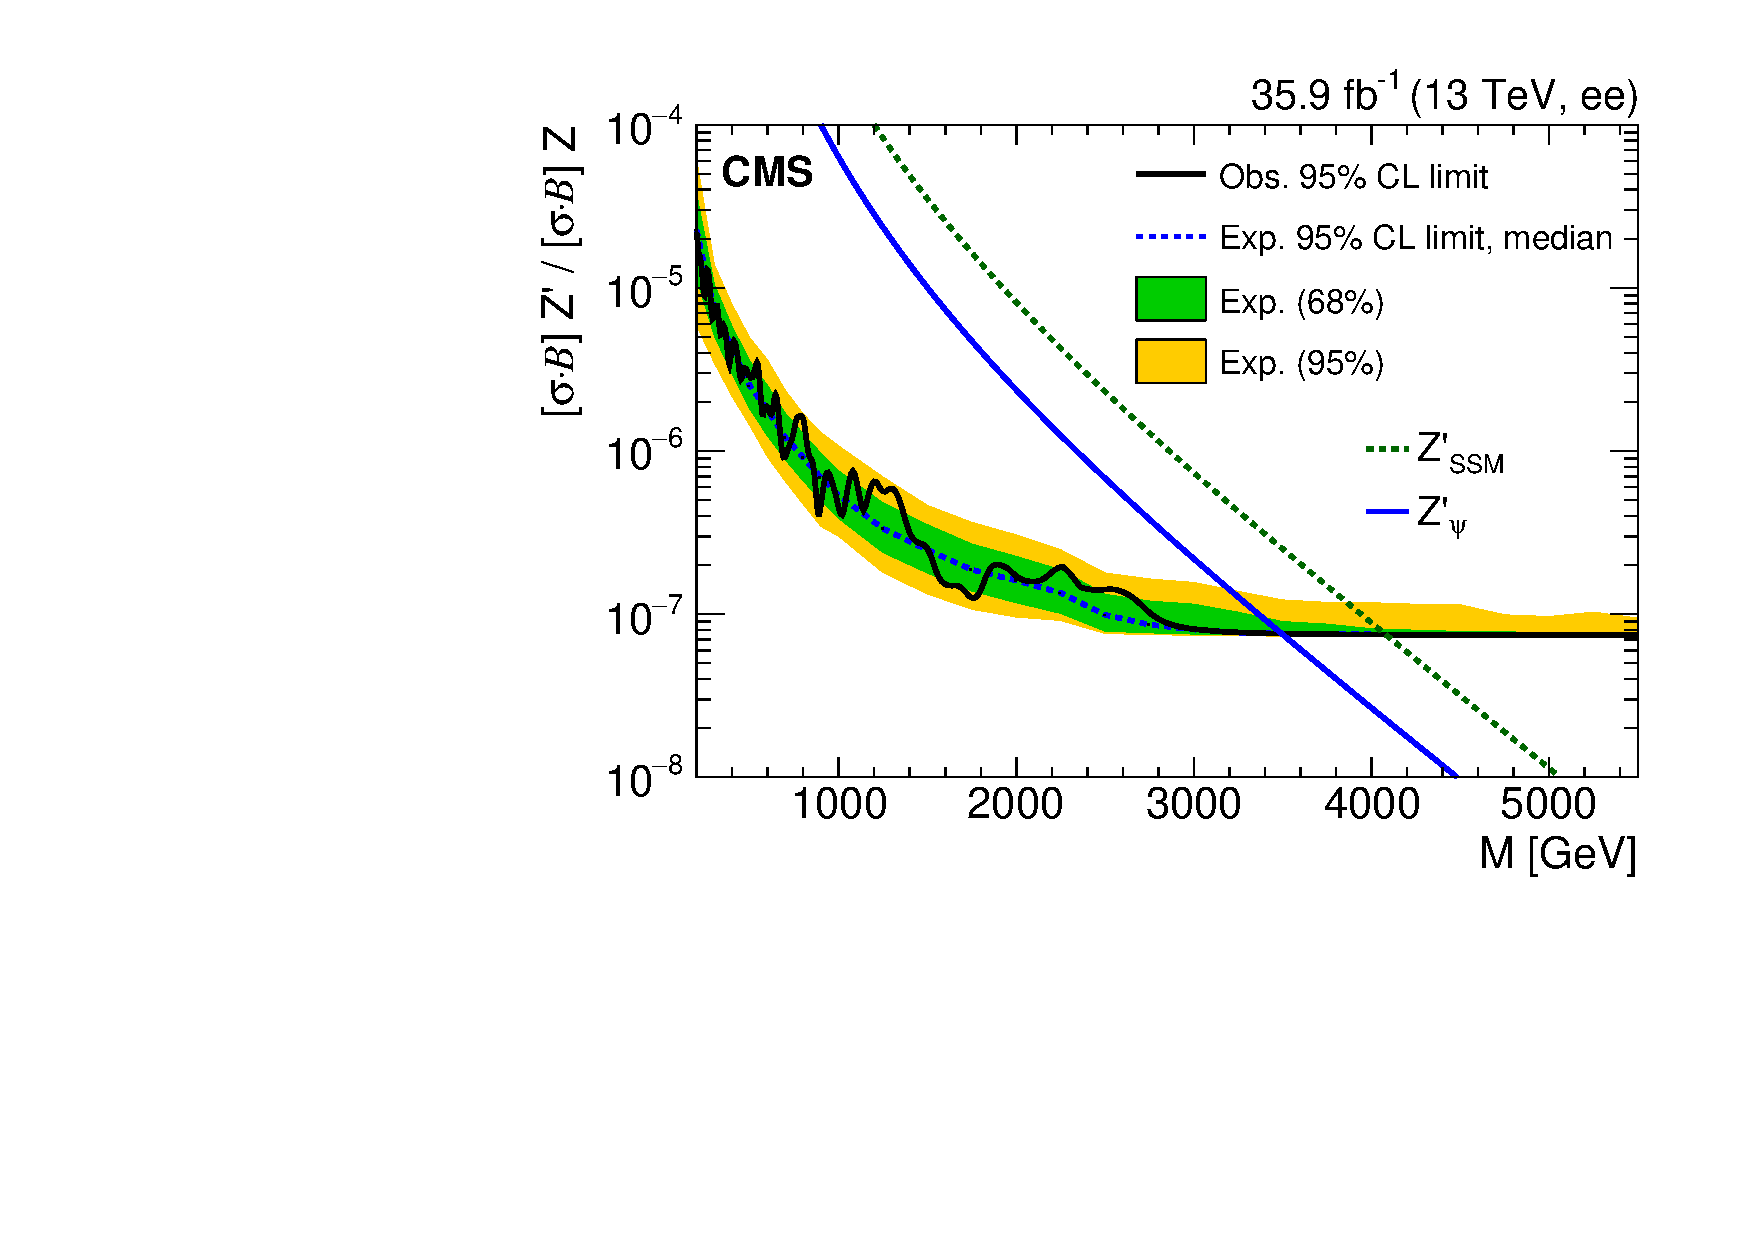
\includegraphics[width=0.47\textwidth]{figures/Zprime/2016/paper/Figure_003-a.pdf}
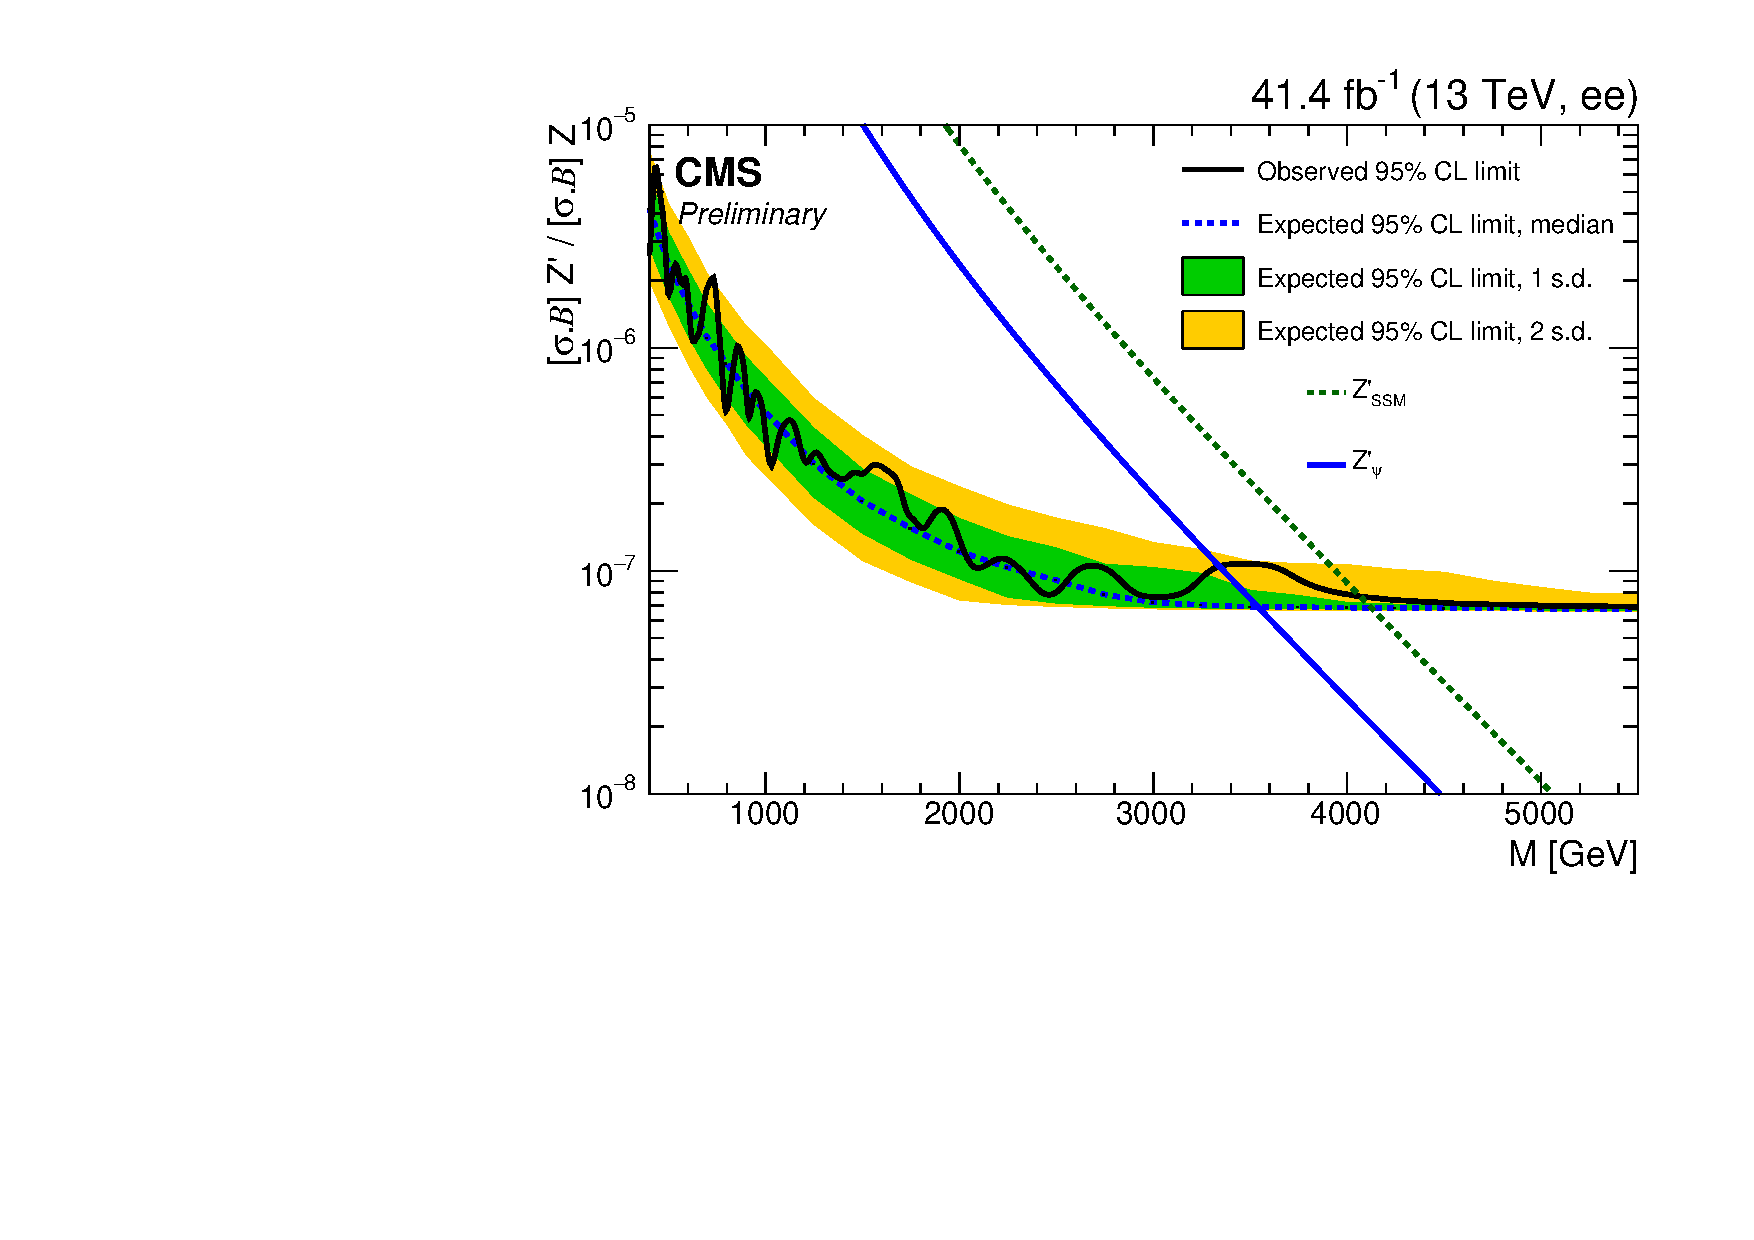
\includegraphics[width=0.47\textwidth]{figures/Zprime/2017/limitInputs/limitPlot_Dielectron2017_forApproval.pdf}
 \caption{The 95\% CL upper limits on $R_\sigma$ for a spin 1 resonance with a width equal to 0.6\% of the resonance mass for 2016 (left) and 2017 (right). The shaded bands correspond to the 68\% and 95\% quantities for the expected limits.  Theoretical predictions for the spin 1 $\ZPSSM$ and $\ZPPSI$ resonances are also shown.}
\label{fig:limit_ee}
\end{figure}

\medskip
In parallel to the search for new resonances in the dielectron final state, a similar search was performed using the dimuon final state \cite{CMS-AN-2016-391}.
Given that the sensitivity of the two searches is comparable and under the assumption that the BR to dielectron and dimuon final state is the same, the upper limits coming from the two separate searches can be combined. The upper limits for the combination of the dielectron (using 2016 and 2017 data) and dimuon (using 2016 data) analysis is shown in Figure \ref{fig:limit_comb}.

\begin{figure}[!htb]
\centering
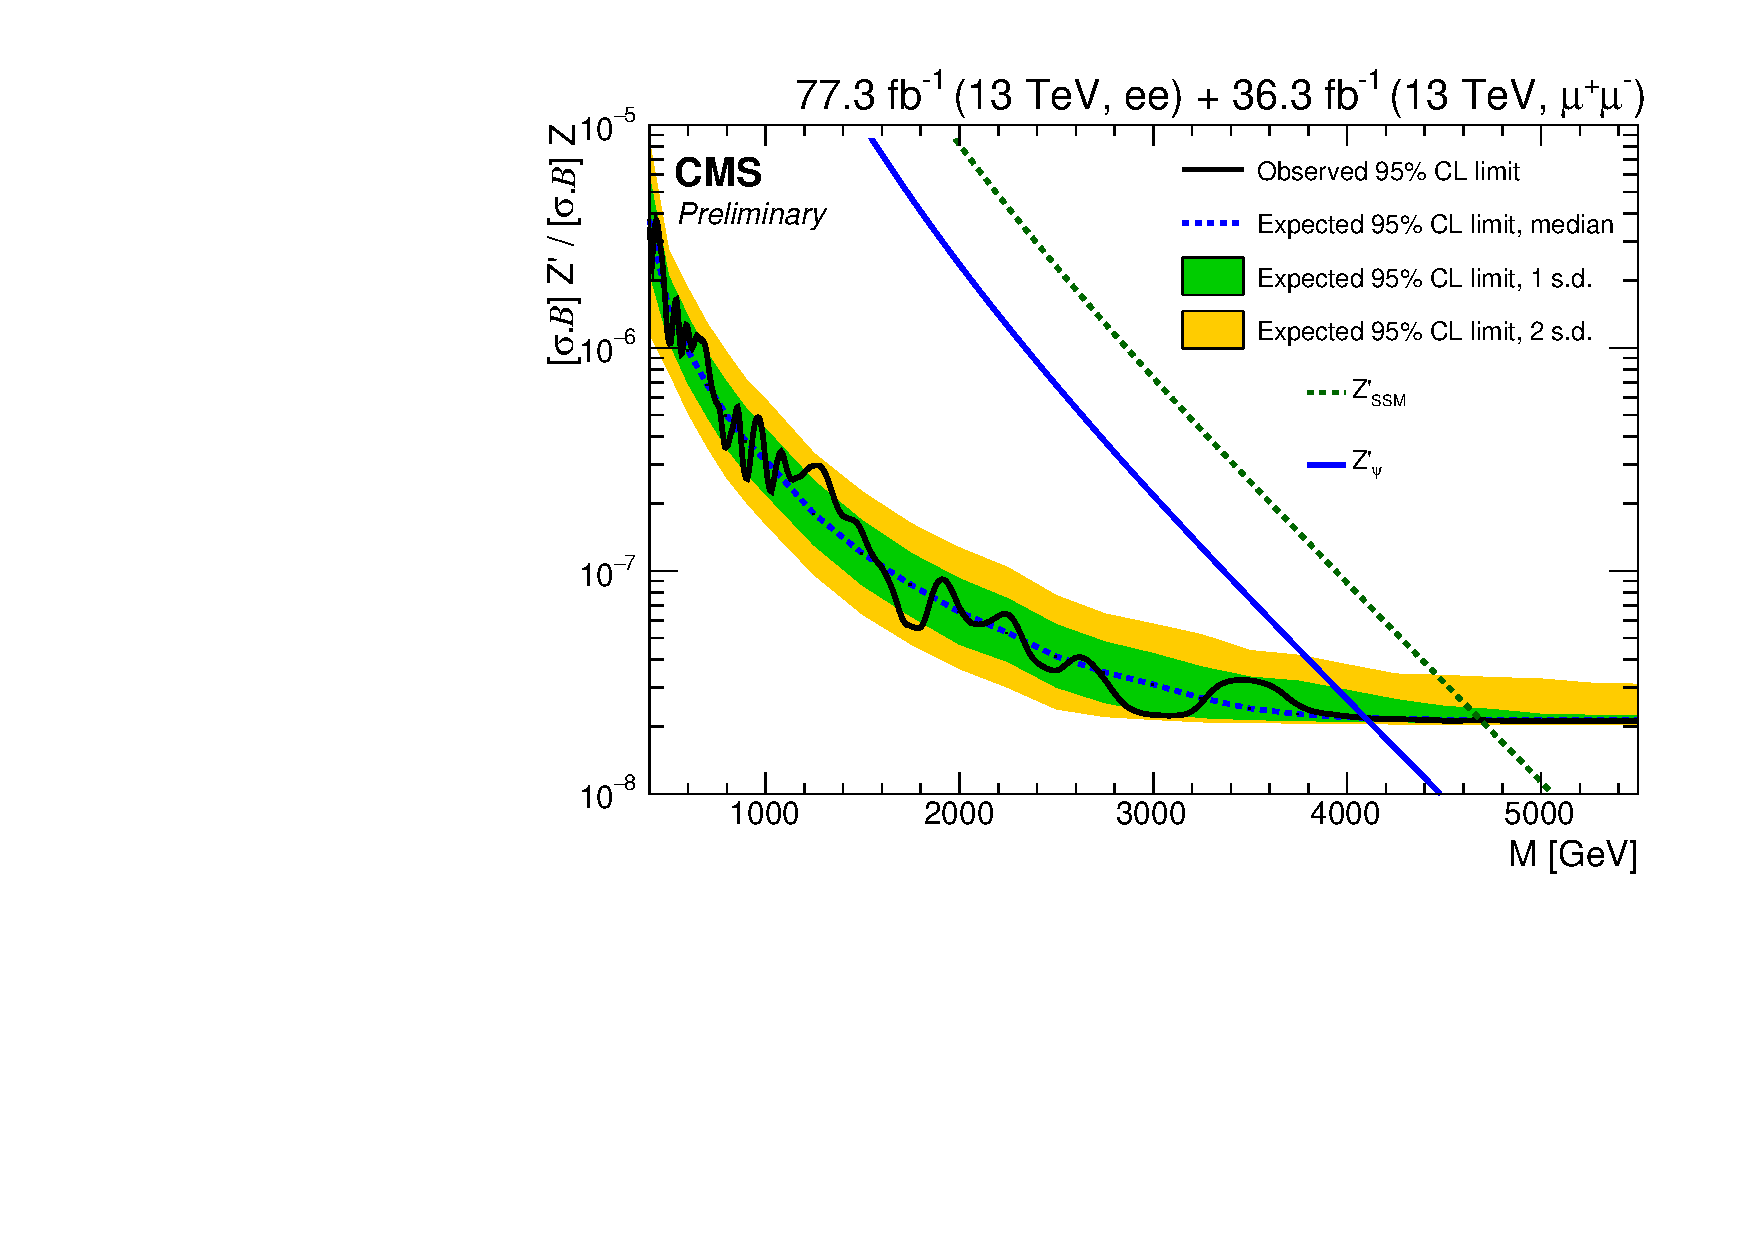
\includegraphics[width=0.7\textwidth]{figures/Zprime/2017/limitInputs/limitPlot_Combination_forApproval.pdf}
 \caption{The 95\% CL upper limits on $R_\sigma$ for a spin 1 resonance with a width equal to 0.6\% of the resonance mass for the dielectron (using 2016 and 2017 data) and dimuon (using 2016 data) final states combined. The shaded bands correspond to the 68\% and 95\% quantities for the expected limits.  Theoretical predictions for the spin 1 $\ZPSSM$ and $\ZPPSI$ resonances are also shown.}
\label{fig:limit_comb}
\end{figure}

In Addition, In 2016 the results for widths equal to 0.6\%, 3\%, 5\% and 10\% of the resonance mass are shown in figure~\ref{fig:limit_ee_width} and one can see at high masses the limits do not exhibit any dependence on the assumed resonance width.
\begin{figure}[!htb]
\centering
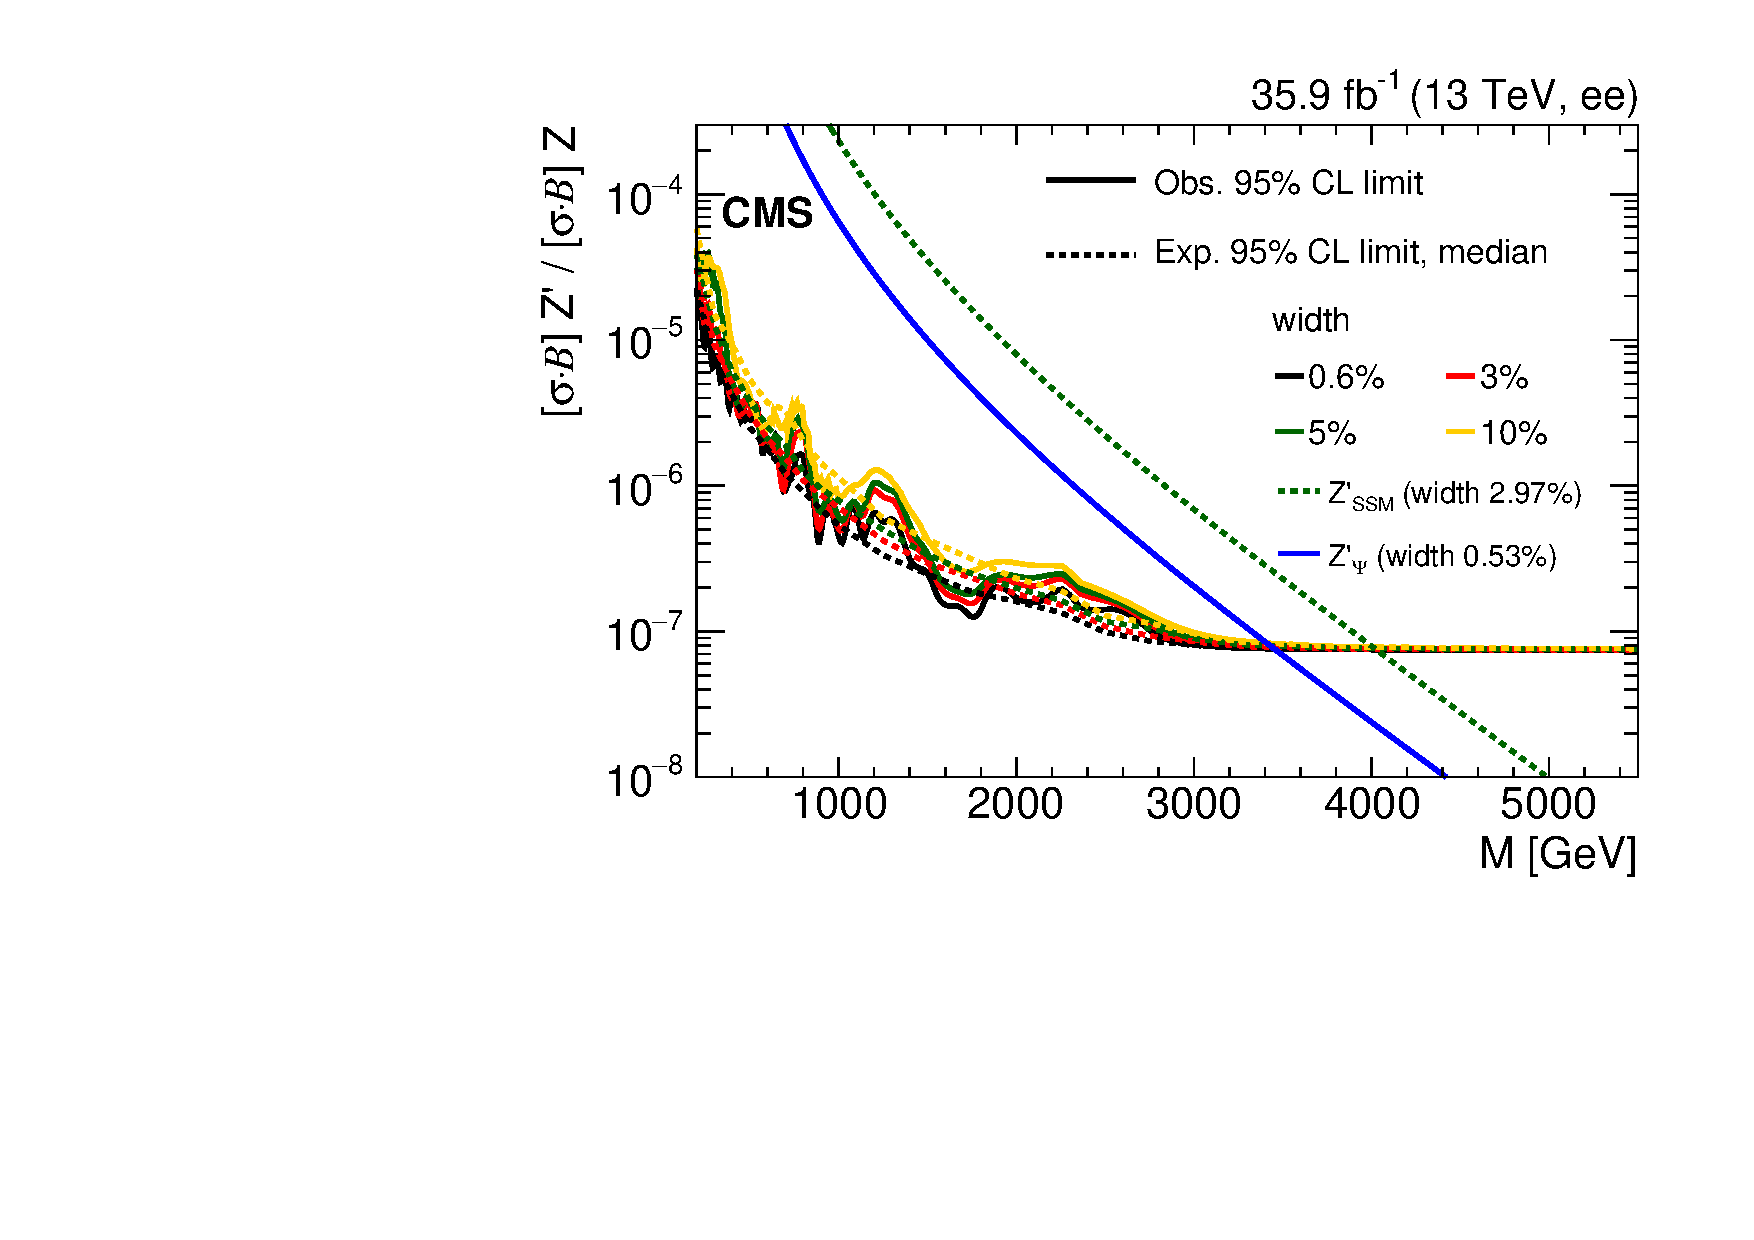
\includegraphics[width=0.7\textwidth]{figures/Zprime/2016/paper/Figure_004-a.pdf}
 \caption{The 95\% CL upper limits on $R_\sigma$ for a spin 1 resonance with a width equal to 0.6\%, 3\%, 5\% and 10\% of the resonance mass in 2016.}
\label{fig:limit_ee_width}
\end{figure}

\medskip
Table \ref{tab:massLimitsSpin1} lists the lower limit on the resonance mass for the $\ZPSSM$ and $\ZPPSI$ models, for the dielectron final states in 2016 and 2017 and for its combination with dimuon final states from 2016.

\begin{table}[!htb]
\begin{center}
\begin{tabular}{|l|c|c|c|c|}
\hline
\multicolumn{1}{|l|}{}  & \multicolumn{2}{c|}{$\ZPSSM$} & \multicolumn{2}{c|}{$\ZPPSI$}  \\
\hline
Channel             & Observed (TeV) & Expected (TeV)      & Observed (TeV)  & Expected (TeV)      \\\hline
ee (2016)           &  4.10      & 4.10            & 3.45        & 3.45            \\
ee (2017)           &  4.10      & 4.15            & 3.35        & 3.55            \\
ee (2016 and 2017) + $\mu\mu$ (2016)        &  4.70      & 4.70            & 4.10        & 4.10            \\
\hline
\end{tabular}
\caption{The observed and expected 95\% CL lower limits on the masses of spin 1 $\ZPSSM$ and $\ZPPSI$ bosons, assuming a signal width of 0.6\% (3\%) of the resonance mass for $\ZPPSI$ ($\ZPSSM$). }
\label{tab:massLimitsSpin1}
\end{center}
\end{table}

Finally, in 2016 the expected and observed limits for a spin-2 resonance with intrinsic widths of 0.01, 0.36, and 1.42 GeV corresponding to coupling parameters $k/\overline{M}_{Pl}$ of 0.01, 0.05, and 0.10 are shown in Figure \ref{fig:limit_spin2} for the dielectron channel and dielectron dimuon combined. Table \ref{tab:massLimitsSpin2} presents the values of the observed and expected 95\% CL lower limits of the aforementioned models.


\begin{figure}[!htb]
\centering
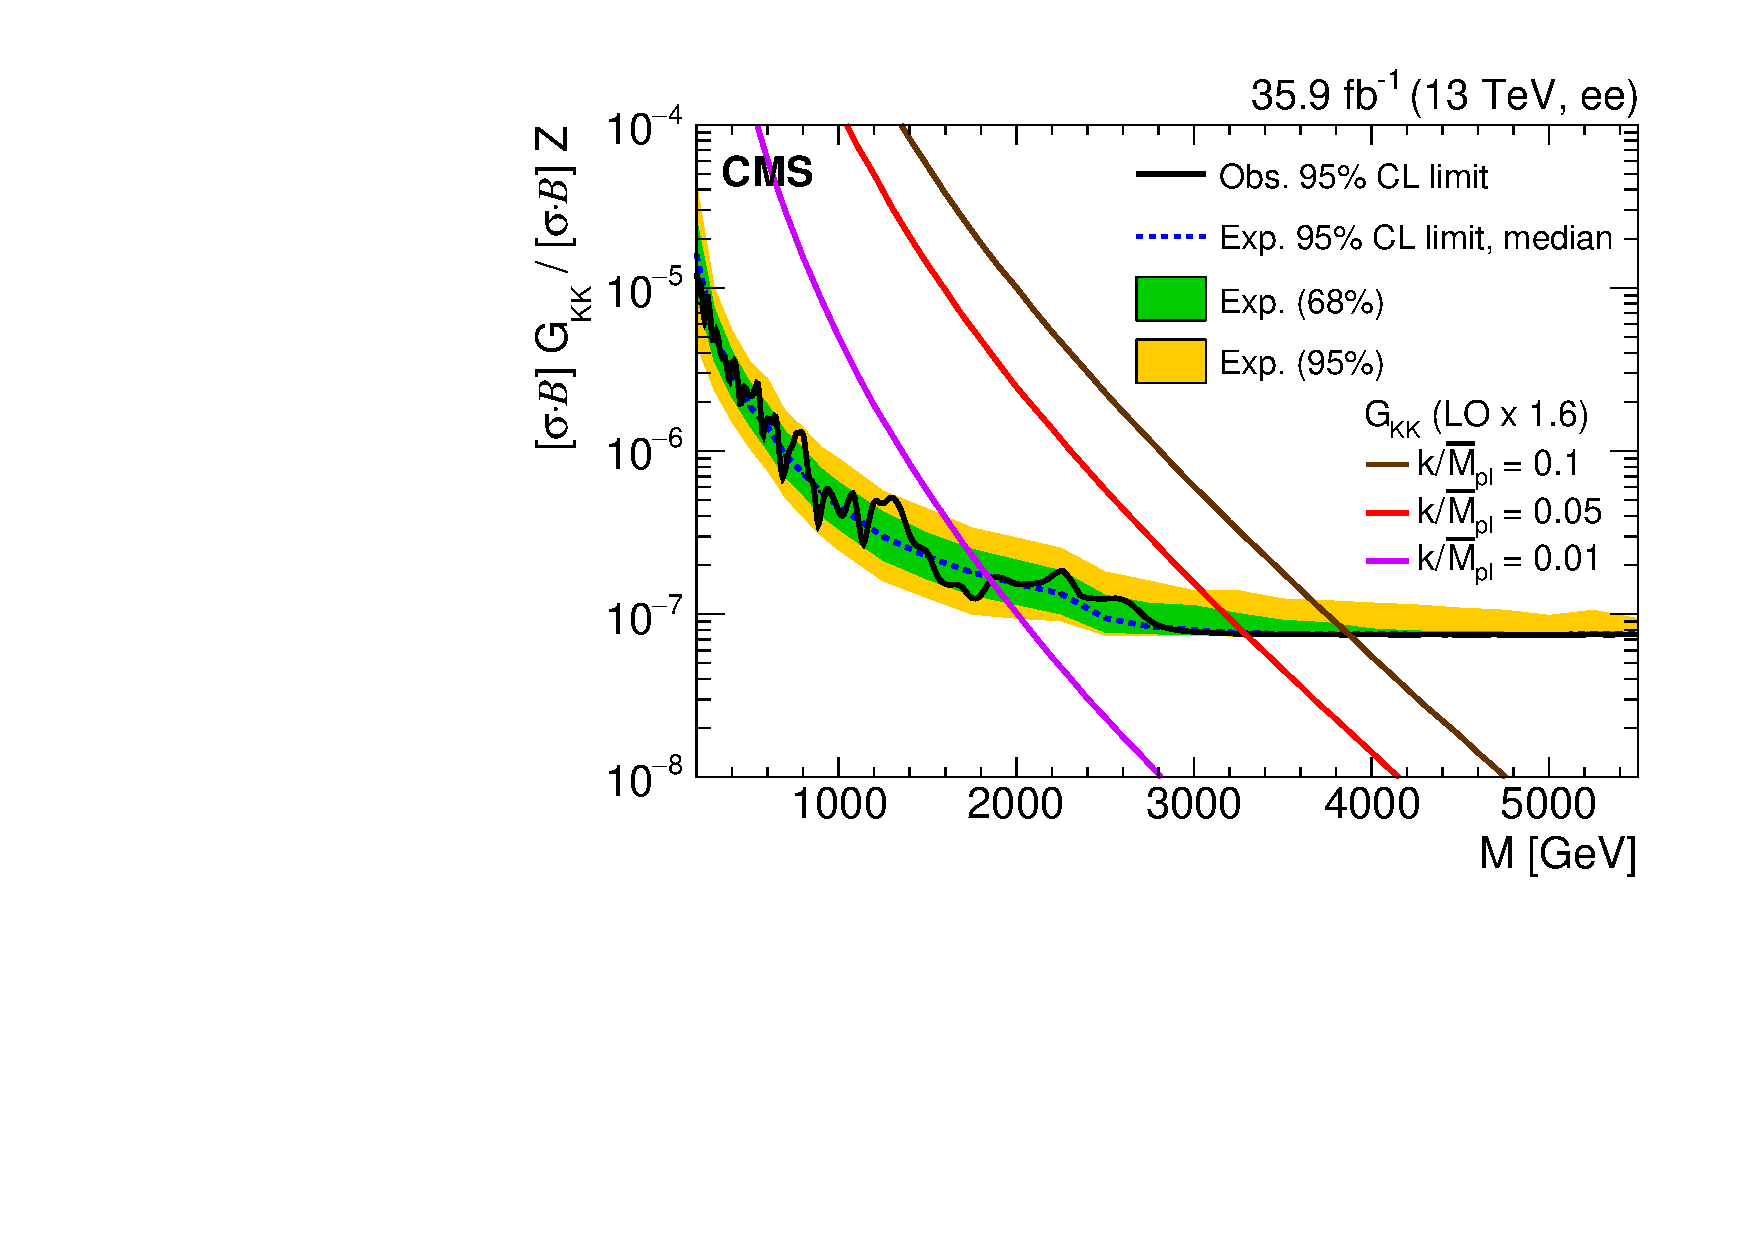
\includegraphics[width=0.47\textwidth]{figures/Zprime/2016/paper/Figure_007-a.pdf}
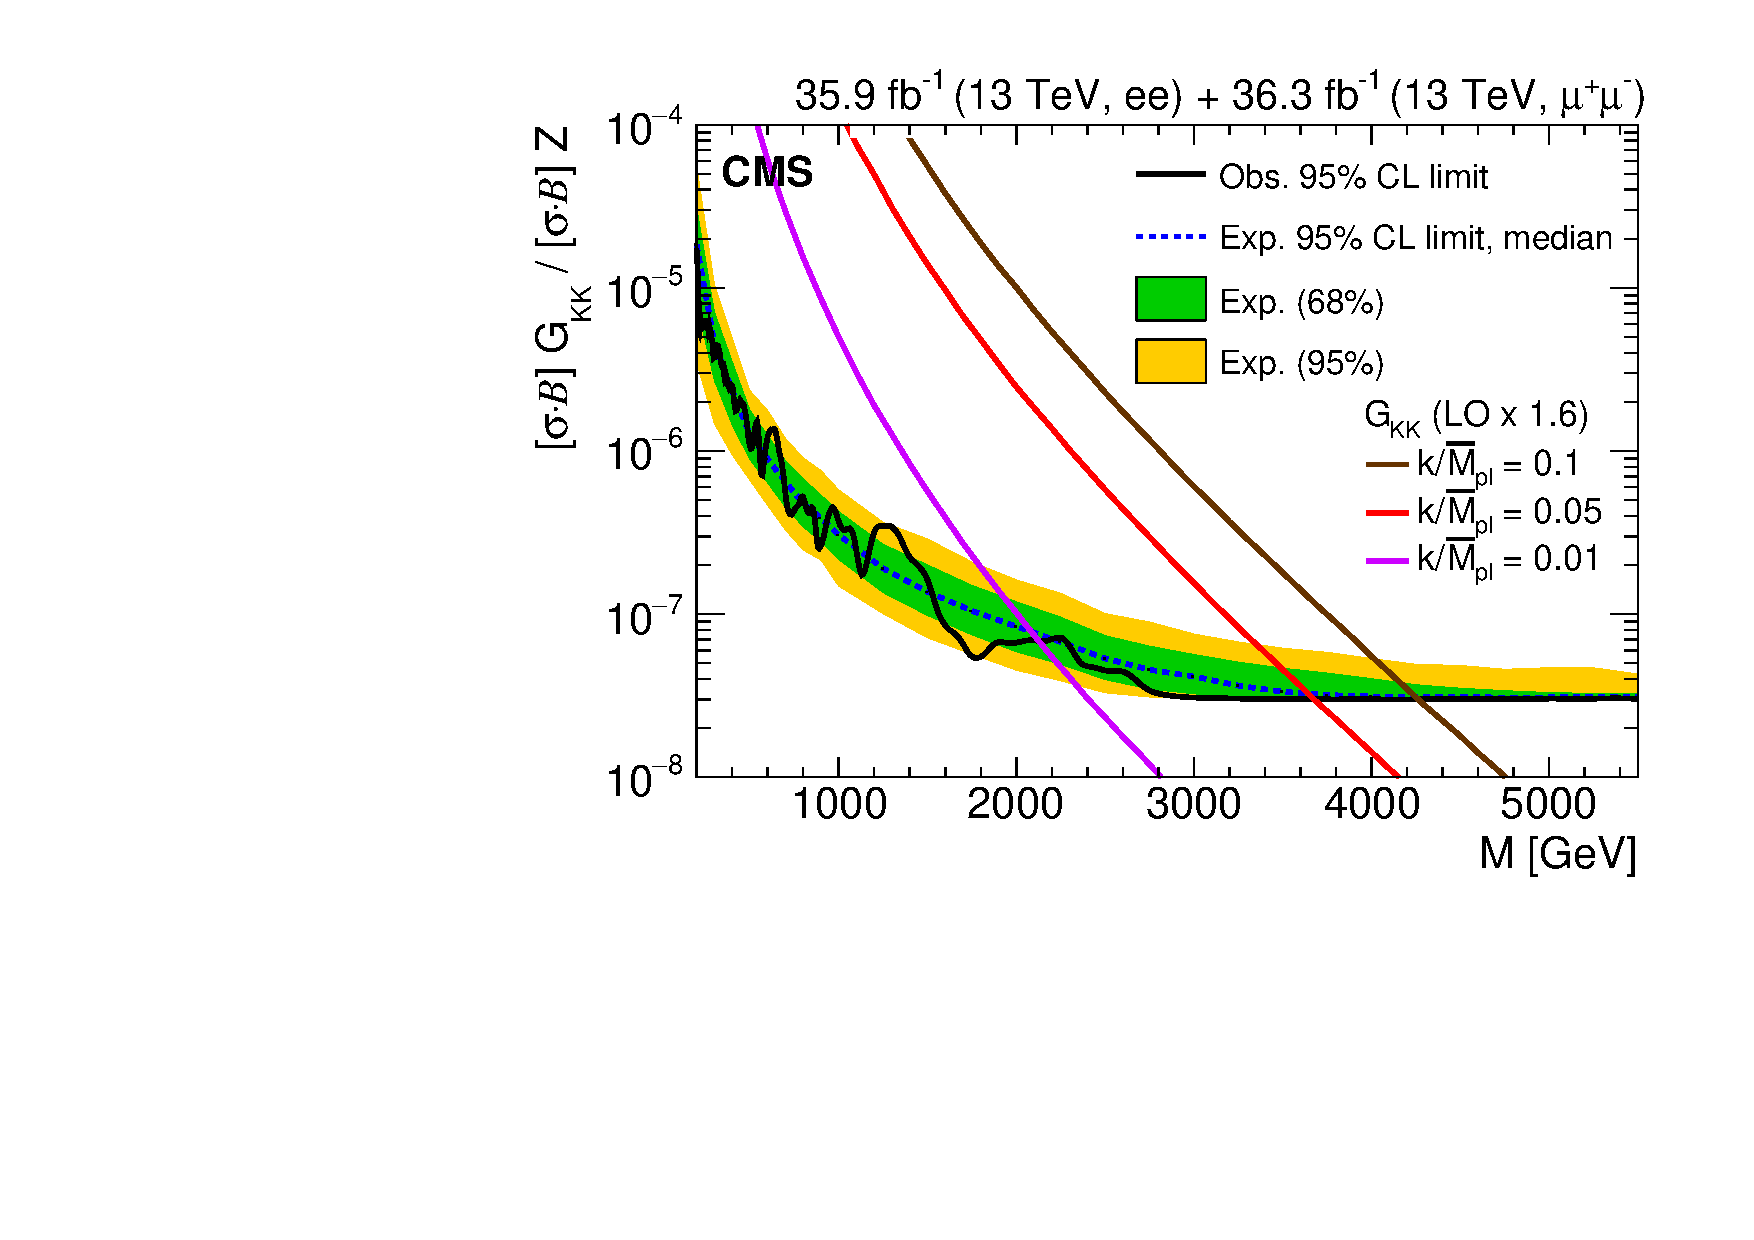
\includegraphics[width=0.47\textwidth]{figures/Zprime/2016/paper/Figure_007-c.pdf}
 \caption{The 95\% CL upper limits on $R_\sigma$ for a spin 2 resonance for the dielectron (left) and its combination with dimuon (right) final states in 2016. The shaded bands correspond to the 68\% and 95\% quantities for the expected limits.  Theoretical predictions for the spin 2 resonances with width equal to 0.01, 0.36 and 1.42 GeV corresponding to coupling parameters $k/\overline{M}_{Pl}$ of 0.01, 0.005 and 0.10 are shown for comparison.}
\label{fig:limit_spin2}
\end{figure}


\begin{table}[!htb]
\begin{center}
\begin{tabular}{|l|c|c|c|c|c|c|}
\hline
\multirow{2}{*}{Channel}  & \multicolumn{2}{c|}{$k/\overline{M}_{Pl}$=0.01} & \multicolumn{2}{c|}{$k/\overline{M}_{Pl}$=0.05} & \multicolumn{2}{c|}{$k/\overline{M}_{Pl}$=0.1}  \\\cline{2-7}
                          & Obs. (TeV) & Exp. (TeV)                         & Obs. (TeV) & Exp. (TeV)                         & Obs. (TeV) & Exp. (TeV)    \\\hline
ee (2016)                 &  1.85      & 1.85                               & 3.30        & 3.30                              & 3.90       & 3.90          \\
ee (2016) + $\mu\mu$ (2016)& 2.10      & 2.05                               & 3.65        & 3.60                              & 4.25       & 4.25          \\
\hline
\end{tabular}
\caption{The observed and expected 95\% CL lower limits on the masses of spin 2 resonance with width equal to 0.01, 0.36 and 1.42 GeV corresponding to coupling parameters $k/\overline{M}_{Pl}$ of 0.01, 0.005 and 0.10.}
\label{tab:massLimitsSpin2}
\end{center}
\end{table}

%\subsection{Motivated models}
%\label{theory:e6}
%
%In the class of models based on the $E_6$ gauge group,
%the unified symmetry group can break to the SM in a number of different ways.
%In many of them, $E_6$ is first broken to $\mathrm{SO}(10) \times \mathrm{U}(1)_\psi$,
%with $\mathrm{SO}(10)$ then breaking either to
%$\mathrm{SU}(4) \times \mathrm{SU}(2)_\mathrm{L} \times \mathrm{SU}(2)_\mathrm{R}$ or $\mathrm{SU}(5) \times \mathrm{U}(1)_\chi$.
%In the $\mathrm{SU}(5)$ case, the presence of $\mathrm{U}(1)_\psi$ and $\mathrm{U}(1)_\chi$ symmetries
%implies the existence of associated gauge bosons \zppsi\ and \zpchi\ that can mix.
%When $\mathrm{SU}(5)$ is broken down to the SM, one of the $\mathrm{U}(1)$ can remain unbroken down
%to intermediate energy scales.
%Therefore, the precise model is governed by a mixing angle $\te6$, with the new
%potentially observable \zp\ boson defined by $\zp(\te6)=\zppsi\cos\te6+\zpchi\sin\te6$.
%The value of $\te6$ specifies the \zp\ boson's coupling strength to SM fermions
%as well as its intrinsic width.
%In comparison to the benchmark \zpssm, which has a width of approximately 3\% of its mass,
%the \esix\ models predict narrower \zp\ signals.
%All other \zp\ signals in this model, including \zpsq, \zpI, \zpeta, and \zpN, are defined by specific values of $\te6$ ranging
%from 0 to $\pi$, and have widths between those of the \zppsi\ and \zpchi.
%
%In Figure \ref{limit}, cross section of considered models as a function of mass are shown. Upper bounds obtained on the cross section times branching ratio for each model are summarized in Table \ref{Z_models}.
%
%\begin{table}[]
%\centering
%\caption{Observed and expected 95\% C.L. lower mass limits for various $Z^{'}$ gauge boson models}
%\label{Z_models}
%\begin{tabular}{|c|c|c|}
%\hline
%Model          & Exp(TeV) & Obs(TeV) \\ \hline
%$Z^{'}_{SSM}$  & 4.02     & 4.00    \\ \hline
%$Z^{'}_{\chi}$ & 3.74    &  3.72   \\ \hline
%$Z^{'}_{S}$    & 3.68    &  3.66   \\ \hline
%$Z^{'}_{I}$    & 3.62    &  3.60   \\ \hline
%$Z^{'}_{N}$    & 3.50    &  3.48   \\ \hline
%$Z^{'}_{\eta}$ & 3.52    &  3.50   \\ \hline
%$Z^{'}_{\psi}$ & 3.44    &  3.42   \\ \hline
%\end{tabular}
%\end{table}
